% master file siminos/froehlich/slice/intro.tex
% $Author$ $Date$

% \section{Introduction}
%    \label{sec:intro}

In spatially extended, turbulent flows one observes similar patterns at
different spatial positions and at different times. How `similar?' If the
flow is equivariant under a group of continuous symmetries, one way of
answering this question is by measuring distances between different
states in the symmetry-reduced \statesp\ $\pS/\Group$, a space in which
each group orbit (class of physically equivalent states) is represented
by a single point. This `distance' depends on the choice of norm and on
the symmetry-reduction method.

													\toCB
In 1980 Phil Morrison\rf{Morr80,Morr98} showed how to derive Hamiltonian
description of ideal fluid (plasma) dynamics from the Low
Lagrangian\rf{Low58} by a transformation from Lagrangian to Eulerian
variables. Morrison's method is an important example of symmetry
reduction: the \statesp\ of time-labeled Lagrangian trajectories of fluid
`particles' is reduced to a much smaller \statesp\ of Eulerian velocity
fields (time independent, if the flow is steady). It is also a very
difficult example of symmetry reduction; the reductions steps have to be
executed judiciously, new variables cleverly chosen, and ``one should do
the Legendre transformations slowly and carefully when there are
degeneracies\rf{CHHM98}.'' Our goal here is different. Rather than to
reduce a particular set of dynamical equations, we seek to formulate a
computationally straightforward general method of reducing continuous
symmetries, applicable to any high-dimensional chaotic/turbulent flow,
such as the fluid flows bounded by pipes or planes. The
symmetry-reduction literature is very extensive (see
\refrefs{CBcontinuous,SiCvi10} for a review), but it basically offers two
approaches (a) invariant polynomial bases, and (b) methods which pick a
representative point by slicing group orbits, generalizing the way in
which {\PoincSec}s cut time-evolving trajectories. For high-dimensional
flows the \mslices\ studied in \refrefs{CBcontinuous,SiCvi10,Wilczak09}
appears to be the only feasible approach, implementable in practice. Here
the method is rederived as a distance minimization problem in the space
of patterns.

The new results reported in this paper are:
    (a) A generic linear slice cuts across group orbits of {\em all}
        states in the \statesp\ (\refsect{sec:frame}).
    (b) Every slice carries along with it a {\sset}. We show how to
        compute the jump of the \reducedsp\ trajectory
         (\refsect{sec:mslices}) whenever it crosses
        through such singularity  (\refsect{sec:singul}).
    (c) We propose to avoid these singularities (artifacts of the symmetry
        reduction by linear slices) by tiling the \statesp\ with an atlas
        constructed from a set of local slices  (\refsect{sec:chart}).
Basic facts about symmetries of dynamical systems are  reviewed in
\refappe{sec:SymmDyn}. In  \refappe{sec:singulProd} we show that for
continuous symmetries with product structure (such as $\SOn{2} \times
\SOn{2}$ symmetries of pipe and plane fluid flows), each symmetry induces
its own {\sset}.

In what follows we denote by `\mframes' the post-processing of the full
\statesp\ flow (\refsect{exam:CLErotAngle}), and by `\mslices' the
integration of flow confined to the \reducedsp\ (\refsect{sec:mslices}).
In practice, symmetry reduction is best carried out as post-processing,
after the numerical trajectory is obtained by integrating the full
\statesp\ flow. In particular, the symmetry-reduction induced
singularities (\refsect{sec:singul}) are more tractable numerically
if given the full \statesp\ trajectory.

 \begin{figure}
 \begin{center}
(a)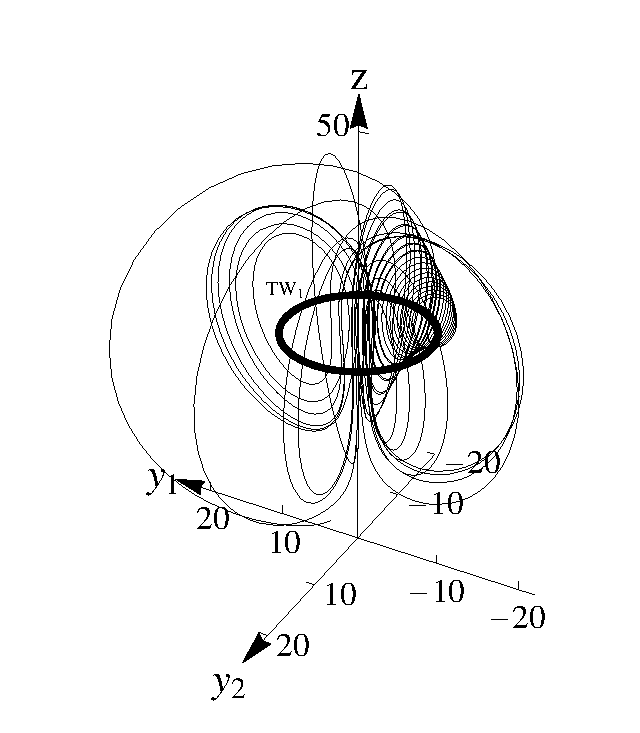
\includegraphics[width=0.45\textwidth]{Fullspace}%
(b)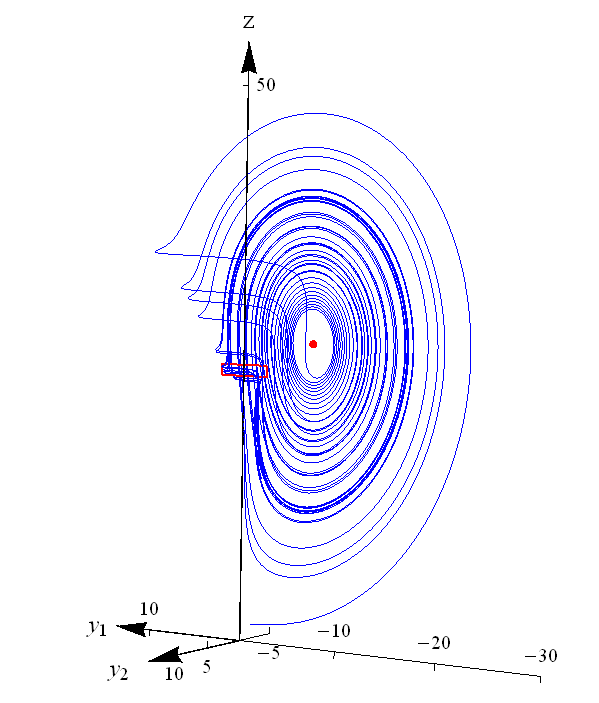
\includegraphics[width=0.38\textwidth]{RedTrajNoPlane1}%
 \end{center}
 \caption{\label{fig:Fullspace}
(color online).
(a) \CLe\ \refeq{eq:CLeR} exhibit a strange attractor for parameter
values \refeq{SiminosPrmts}, here projected on the $\{y_1,y_2,z\}$ axes.
(thin line/blue) A segment of generic finite time trajectory.
(thick line/red)
$\REQV{}{1}$, the only \reqv.
%
% Former {CLEreduced} \label{fig:RedTrajNoPlane1}
(b) The same strange attractor plotted in the symmetry-\reducedsp\
% with initial point
%$(x_1, x_2, y_1, y_2, z) = (1, 2, 3, 1, 2)$
in the slice \refeq{PCsectQ0}, defined by the group tangent
$\sliceTan{}$ whose choice is explained in \refeq{exmplTempl}.
In the \reducedsp\ \reqv\ $\REQV{}{1}$ is reduced to \eqv\ $\EQV{1}$.
Note, however, the semicircular jumps in the reduced flow. These are
analyzed in \refsect{sec:singul}. For a blow-up of the jump
indicted by the small rectangle (red), see \reffig{fig:singpass}.
 }%
 \end{figure}

We shall illustrate symmetry reduction by applying it to the
5-dimensional \cLe\rf{GibMcCLE82}
\bea
	\dot{x}_1 &=& -\sigma x_1 + \sigma y_1
\,,\qquad\qquad\qquad
	\dot{x}_2 \,=\, -\sigma x_2 + \sigma y_2
\continue
	\dot{y}_1 &=& (r_1-z)\, x_1  - ~y_1 - e y_2
\,,\qquad\;
	\dot{y}_2 \,=\, (r_1-z)\, x_2 + e y_1 - ~y_2
\label{eq:CLeR}\\
	\dot{z}~ &=& -b z + x_1 y_1 + x_2 y_2
\,.
\nnu
\eea
In all numerical calculations that follow we shall set the
parameters to \refref{SiCvi10} values,
\beq
r_1=28,\; b={8}/{3},\;
\sigma=10,\quad \mbox{and}  \quad e={1}/{10}
\,,
\ee{SiminosPrmts}
for which the flow exhibits a strange attractor,
\reffig{fig:Fullspace}\,(a).
\CLe\ are a simple example of a dynamical system
with a continuous (but no discrete) symmetry.
They are equivariant \refeq{eq:FiniteRot} under \SOn{2} rotations by
	\ifarticle  %submission version
\bea
\LieEl(\gSpace)
    &=&
\exp{({\gSpace} \cdot \Lg)}
	 \,=\,
  \left(\barr{ccccc}
  \cos \gSpace  & \sin \gSpace  & 0 & 0 & 0 \\
 -\sin \gSpace  & \cos \gSpace  & 0 & 0 & 0 \\
 0 & 0 &  \cos \gSpace & \sin \gSpace   & 0 \\
 0 & 0 & -\sin \gSpace & \cos \gSpace   & 0 \\
 0 & 0 & 0             & 0              & 1
    \earr\right)
\continue
\Lg &=&
   \left(\barr{ccccc}
    0  &  1 & 0  &  0 & 0  \\
   -1  &  0 & 0  &  0 & 0 \\
    0  &  0 & 0  &  1 & 0  \\
    0  &  0 &-1  &  0 & 0 \\
    0  &  0 & 0  &  0 & 0
    \earr\right)
% \,.
\label{CLfRots}
\eea
    \else  %web version
\bea
\LieEl(\gSpace)
    &=&
\exp{({\gSpace} \cdot \Lg)}
	 \,=\,
  \left(\barr{ccccc}
  \cos \gSpace  & \sin \gSpace  & 0 & 0 & 0 \\
 -\sin \gSpace  & \cos \gSpace  & 0 & 0 & 0 \\
 0 & 0 &  \cos \gSpace & \sin \gSpace   & 0 \\
 0 & 0 & -\sin \gSpace & \cos \gSpace   & 0 \\
 0 & 0 & 0             & 0              & 1
    \earr\right)
\,,\qquad \Lg \,=\,
   \left(\barr{ccccc}
    0  &  1 & 0  &  0 & 0  \\
   -1  &  0 & 0  &  0 & 0 \\
    0  &  0 & 0  &  1 & 0  \\
    0  &  0 &-1  &  0 & 0 \\
    0  &  0 & 0  &  0 & 0
    \earr\right)
% \,.
\label{CLfRots}
\eea
	\fi
(for group-theoretical notation, see \refappe{sec:SymmDyn}). The group is
1\dmn\ and compact, its elements parameterized by $\gSpace \mbox{ mod }
2\pi$. The fixed-point subspace \refeq{dscr:InvPoints} is the $z$-axis.
The velocity \refeq{eq:CLeR} at a point on the $z$-axis points only in
the $z$-direction and so the trajectory remains on the $z$-axis for all
times. The action of \SOn{2}\ thus decomposes the  \statesp\ into $m=0$
\SOn{2}-invariant subspace ($z$-axis) and  $m=1$ subspace of multiplicity
2. Locally, at \statesp\ point $\ssp$, the infinitesimal action of the
group is given by the group tangent field $\groupTan(\ssp) = \Lg \ssp =
(x_2,-x_1,y_2,-y_1,0)$, with the flow induced by the group action normal
to the radial direction in the $(x_1,x_2)$ and $(y_1,y_2)$ planes, while
the $z$-axis is left invariant.

%
% ****** End of file intro.tex ******
